\documentclass[letterpaper]{article}
\usepackage[submission]{aaai2027}
\usepackage{times}
\usepackage{helvet}
\usepackage{courier}
\usepackage[hyphens]{url}
\usepackage{graphicx}
\urlstyle{rm}
\def\UrlFont{\rm}
\usepackage{natbib}
\usepackage{caption}
\frenchspacing
\setlength{\pdfpagewidth}{8.5in}
\setlength{\pdfpageheight}{11in}
\usepackage{amsmath}
\usepackage{amssymb}
\usepackage{amsthm}
\usepackage{booktabs}
\renewcommand{\arraystretch}{0.92}
\newcommand{\LSTMauroc}{0.9558}
\newcommand{\LSTMaurocCI}{[0.9446, 0.9662]}
\newcommand{\LSTMf}{0.905}
\newcommand{\LSTMfCI}{[0.886, 0.920]}
\newcommand{\LSTMprec}{0.893}
\newcommand{\LSTMprecCI}{[0.866, 0.917]}
\newcommand{\LSTMrec}{0.916}
\newcommand{\LSTMrecCI}{[0.894, 0.937]}
\newcommand{\LSTMacc}{0.900}
\newcommand{\LSTMaccCI}{[0.883, 0.917]}
\newcommand{\LSTMfp}{63}
\newcommand{\LSTMfn}{48}
\newcommand{\GRUauroc}{0.9712}
\newcommand{\GRUaurocCI}{[0.9623, 0.9795]}
\newcommand{\GRUf}{0.920}
\newcommand{\GRUfCI}{[0.903, 0.937]}
\newcommand{\GRUprec}{0.913}
\newcommand{\GRUprecCI}{[0.890, 0.936]}
\newcommand{\GRUrec}{0.927}
\newcommand{\GRUrecCI}{[0.905, 0.946]}
\newcommand{\GRUacc}{0.917}
\newcommand{\GRUaccCI}{[0.900, 0.934]}
\newcommand{\GRUfp}{51}
\newcommand{\GRUfn}{42}
\newcommand{\Transformerauroc}{0.9810}
\newcommand{\TransformeraurocCI}{[0.9749, 0.9872]}
\newcommand{\Transformerf}{0.940}
\newcommand{\TransformerfCI}{[0.926, 0.954]}
\newcommand{\Transformerprec}{0.947}
\newcommand{\TransformerprecCI}{[0.929, 0.964]}
\newcommand{\Transformerrec}{0.934}
\newcommand{\TransformerrecCI}{[0.913, 0.953]}
\newcommand{\Transformeracc}{0.939}
\newcommand{\TransformeraccCI}{[0.925, 0.952]}
\newcommand{\Transformerfp}{30}
\newcommand{\Transformerfn}{38}
\newcommand{\SimpleSTGCNauroc}{0.9185}
\newcommand{\SimpleSTGCNaurocCI}{[0.9016, 0.9340]}
\newcommand{\SimpleSTGCNf}{0.849}
\newcommand{\SimpleSTGCNfCI}{[0.826, 0.870]}
\newcommand{\SimpleSTGCNprec}{0.851}
\newcommand{\SimpleSTGCNprecCI}{[0.822, 0.879]}
\newcommand{\SimpleSTGCNrec}{0.847}
\newcommand{\SimpleSTGCNrecCI}{[0.816, 0.877]}
\newcommand{\SimpleSTGCNacc}{0.845}
\newcommand{\SimpleSTGCNaccCI}{[0.823, 0.865]}
\newcommand{\SimpleSTGCNfp}{85}
\newcommand{\SimpleSTGCNfn}{88}
\newcommand{\MiniROCKETauroc}{0.9760}
\newcommand{\MiniROCKETaurocCI}{[0.9672, 0.9839]}
\newcommand{\MiniROCKETf}{0.936}
\newcommand{\MiniROCKETfCI}{[0.921, 0.950]}
\newcommand{\MiniROCKETprec}{0.931}
\newcommand{\MiniROCKETprecCI}{[0.910, 0.952]}
\newcommand{\MiniROCKETrec}{0.941}
\newcommand{\MiniROCKETrecCI}{[0.920, 0.960]}
\newcommand{\MiniROCKETacc}{0.934}
\newcommand{\MiniROCKETaccCI}{[0.918, 0.948]}
\newcommand{\MiniROCKETfp}{40}
\newcommand{\MiniROCKETfn}{34}
\newcommand{\DTSLRauroc}{0.9433}
\newcommand{\DTSLRaurocCI}{[0.9297, 0.9559]}
\newcommand{\DTSLRf}{0.890}
\newcommand{\DTSLRfCI}{[0.871, 0.909]}
\newcommand{\DTSLRprec}{0.883}
\newcommand{\DTSLRprecCI}{[0.858, 0.906]}
\newcommand{\DTSLRrec}{0.897}
\newcommand{\DTSLRrecCI}{[0.874, 0.922]}
\newcommand{\DTSLRacc}{0.886}
\newcommand{\DTSLRaccCI}{[0.867, 0.905]}
\newcommand{\DTSLRfp}{68}
\newcommand{\DTSLRfn}{59}
\newcommand{\DTSETauroc}{0.9801}
\newcommand{\DTSETaurocCI}{[0.9734, 0.9861]}
\newcommand{\DTSETf}{0.936}
\newcommand{\DTSETfCI}{[0.921, 0.950]}
\newcommand{\DTSETprec}{0.907}
\newcommand{\DTSETprecCI}{[0.883, 0.931]}
\newcommand{\DTSETrec}{0.967}
\newcommand{\DTSETrecCI}{[0.952, 0.980]}
\newcommand{\DTSETacc}{0.932}
\newcommand{\DTSETaccCI}{[0.917, 0.946]}
\newcommand{\DTSETfp}{57}
\newcommand{\DTSETfn}{19}
\newcommand{\DTSRFauroc}{0.9785}
\newcommand{\DTSRFaurocCI}{[0.9711, 0.9849]}
\newcommand{\DTSRFf}{0.927}
\newcommand{\DTSRFfCI}{[0.912, 0.941]}
\newcommand{\DTSRFprec}{0.893}
\newcommand{\DTSRFprecCI}{[0.870, 0.917]}
\newcommand{\DTSRFrec}{0.963}
\newcommand{\DTSRFrecCI}{[0.946, 0.978]}
\newcommand{\DTSRFacc}{0.922}
\newcommand{\DTSRFaccCI}{[0.906, 0.937]}
\newcommand{\DTSRFfp}{66}
\newcommand{\DTSRFfn}{21}
\newcommand{\DTSHGBauroc}{0.9895}
\newcommand{\DTSHGBaurocCI}{[0.9851, 0.9935]}
\newcommand{\DTSHGBf}{0.951}
\newcommand{\DTSHGBfCI}{[0.938, 0.963]}
\newcommand{\DTSHGBprec}{0.934}
\newcommand{\DTSHGBprecCI}{[0.913, 0.954]}
\newcommand{\DTSHGBrec}{0.969}
\newcommand{\DTSHGBrecCI}{[0.953, 0.983]}
\newcommand{\DTSHGBacc}{0.949}
\newcommand{\DTSHGBaccCI}{[0.935, 0.961]}
\newcommand{\DTSHGBfp}{39}
\newcommand{\DTSHGBfn}{18}
\newcommand{\DTSNetauroc}{0.9775}
\newcommand{\DTSNetaurocCI}{[0.9699, 0.9849]}
\newcommand{\DTSNetf}{0.928}
\newcommand{\DTSNetfCI}{[0.911, 0.943]}
\newcommand{\DTSNetprec}{0.927}
\newcommand{\DTSNetprecCI}{[0.907, 0.949]}
\newcommand{\DTSNetrec}{0.929}
\newcommand{\DTSNetrecCI}{[0.907, 0.949]}
\newcommand{\DTSNetacc}{0.926}
\newcommand{\DTSNetaccCI}{[0.909, 0.941]}
\newcommand{\DTSNetfp}{42}
\newcommand{\DTSNetfn}{41}
\newcommand{\bestmodel}{DTSHGB}
\newcommand{\hgbminusrocketauroc}{0.0135}
\newcommand{\hgbminusgcnauroc}{0.0710}
\newcommand{\hgbminusgcnrec}{-0.002}
\newcommand{\hgberr}{0.051}
\newcommand{\gapfactor}{5.6}
\newcommand{\lstmparams}{216{,}193}
\newcommand{\gcnparams}{244{,}161}
\newcommand{\dtsnetparams}{10{,}506}
\newcommand{\nstar}{17{,}599}
\newcommand{\nstarover}{4.9}
\newcommand{\xone}{-0.498}
\newcommand{\xtwo}{0.308}
\newcommand{\pmissf}{0.202}
\newcommand{\pfalsen}{0.369}
\newcommand{\epsqda}{0.286}
\newcommand{\muf}{0.171}
\newcommand{\mun}{0.381}
\newcommand{\sigf}{0.165}
\newcommand{\sign}{0.220}
\newcommand{\lsoOneauroc}{0.9382}
\newcommand{\lsoOneaurocCI}{[0.9259, 0.9492]}
\newcommand{\lsoOnef}{0.866}
\newcommand{\lsoOnefCI}{[0.847, 0.884]}
\newcommand{\lsoOnerec}{0.944}
\newcommand{\lsoOnerecCI}{[0.939, 0.969]}
\newcommand{\lsoOnen}{1{,}513}
\newcommand{\lsoOnefalls}{679}
\newcommand{\lsoTwoauroc}{0.9926}
\newcommand{\lsoTwoaurocCI}{[0.9898, 0.9951]}
\newcommand{\lsoTwof}{0.966}
\newcommand{\lsoTwofCI}{[0.958, 0.973]}
\newcommand{\lsoTworec}{0.954}
\newcommand{\lsoTworecCI}{[0.903, 0.935]}
\newcommand{\lsoTwon}{1{,}593}
\newcommand{\lsoTwofalls}{1{,}072}
\newcommand{\lsoThreeauroc}{0.9840}
\newcommand{\lsoThreeaurocCI}{[0.9797, 0.9879]}
\newcommand{\lsoThreef}{0.925}
\newcommand{\lsoThreefCI}{[0.912, 0.937]}
\newcommand{\lsoThreerec}{0.925}
\newcommand{\lsoThreerecCI}{[0.941, 0.967]}
\newcommand{\lsoThreen}{2{,}064}
\newcommand{\lsoThreefalls}{903}
\newcommand{\lsoFourauroc}{0.9448}
\newcommand{\lsoFouraurocCI}{[0.9227, 0.9645]}
\newcommand{\lsoFourf}{0.868}
\newcommand{\lsoFourfCI}{[0.836, 0.900]}
\newcommand{\lsoFourrec}{0.953}
\newcommand{\lsoFourrecCI}{[0.934, 0.986]}
\newcommand{\lsoFourn}{402}
\newcommand{\lsoFourfalls}{213}
\newcommand{\lsomeanauroc}{0.9649}
\newcommand{\lsomeanf}{0.906}
\newcommand{\lsorangelow}{0.9382}
\newcommand{\lsorangehigh}{0.9926}
\newcommand{\lfoBedauroc}{0.7123}
\newcommand{\lfoBedaurocCI}{[0.6868, 0.7357]}
\newcommand{\lfoBedf}{0.768}
\newcommand{\lfoBedfCI}{[0.749, 0.788]}
\newcommand{\lfoBedn}{1{,}747}
\newcommand{\lfoBedfalls}{922}
\newcommand{\lfoChairauroc}{0.9844}
\newcommand{\lfoChairaurocCI}{[0.9799, 0.9883]}
\newcommand{\lfoChairf}{0.934}
\newcommand{\lfoChairfCI}{[0.923, 0.944]}
\newcommand{\lfoChairn}{1{,}878}
\newcommand{\lfoChairfalls}{961}
\newcommand{\lfoStandauroc}{0.9916}
\newcommand{\lfoStandaurocCI}{[0.9886, 0.9945]}
\newcommand{\lfoStandf}{0.937}
\newcommand{\lfoStandfCI}{[0.926, 0.949]}
\newcommand{\lfoStandn}{1{,}947}
\newcommand{\lfoStandfalls}{984}
\newcommand{\lfomeanauroc}{0.8961}
\newcommand{\lfomeanf}{0.880}
\newcommand{\iidreff}{0.950}
\newcommand{\transfergap}{0.071}
\newcommand{\urfdauroc}{0.9200}
\newcommand{\urfdaurocCI}{[0.8483, 0.9917]}
\newcommand{\urfdrec}{1.000}
\newcommand{\urfdrecCI}{[1.000, 1.000]}
\newcommand{\urfdprec}{0.508}
\newcommand{\urfdprecCI}{[0.379, 0.638]}
\newcommand{\urfdf}{0.674}
\newcommand{\urfdfCI}{[0.550, 0.779]}
\newcommand{\urfdfp}{29}
\newcommand{\urfdfn}{0}
\newcommand{\abFullf}{0.951}
\newcommand{\abFullauroc}{0.9895}
\newcommand{\abBBoxWf}{0.942}
\newcommand{\abBBoxWauroc}{0.9882}
\newcommand{\abBBoxWdf}{-0.009}
\newcommand{\abBBoxWda}{-0.0013}
\newcommand{\abHipYf}{0.939}
\newcommand{\abHipYauroc}{0.9855}
\newcommand{\abHipYdf}{-0.012}
\newcommand{\abHipYda}{-0.0039}
\newcommand{\abTorsoAngf}{0.945}
\newcommand{\abTorsoAngauroc}{0.9892}
\newcommand{\abTorsoAngdf}{-0.006}
\newcommand{\abTorsoAngda}{-0.0003}
\newcommand{\abHipSpdf}{0.949}
\newcommand{\abHipSpdauroc}{0.9897}
\newcommand{\abHipSpddf}{-0.002}
\newcommand{\abHipSpdda}{+0.0002}
\newcommand{\abCtrSpdf}{0.949}
\newcommand{\abCtrSpdauroc}{0.9904}
\newcommand{\abCtrSpddf}{-0.002}
\newcommand{\abCtrSpdda}{+0.0009}
\newcommand{\abHipAccf}{0.947}
\newcommand{\abHipAccauroc}{0.9894}
\newcommand{\abHipAccdf}{-0.004}
\newcommand{\abHipAccda}{-0.0001}
\newcommand{\abShldrYf}{0.943}
\newcommand{\abShldrYauroc}{0.9882}
\newcommand{\abShldrYdf}{-0.008}
\newcommand{\abShldrYda}{-0.0012}
\newcommand{\abHeadYf}{0.951}
\newcommand{\abHeadYauroc}{0.9903}
\newcommand{\abHeadYdf}{-0.001}
\newcommand{\abHeadYda}{+0.0008}
\newcommand{\abStaticf}{0.939}
\newcommand{\abStaticauroc}{0.9872}
\newcommand{\abStaticdf}{-0.012}
\newcommand{\abStaticda}{-0.0023}
\newcommand{\synthcv}{1.000}
\newcommand{\synthdtsathundred}{1.000}
\newcommand{\synthalphamin}{0.996}
\newcommand{\synthbof}{0.500}
\newcommand{\synthdropfour}{1.000}
\newcommand{\synthkeeptwo}{1.000}
\newcommand{\synthalphaonly}{1.000}
\newcommand{\synthdropone}{1.000}
\newcommand{\synthdroptwo}{1.000}
\newcommand{\attnr}{0.650}
\newcommand{\attnp}{0.081}
\newcommand{\attntopfam}{Head-Y}
\newcommand{\attntopw}{0.148}
\newcommand{\attntopei}{0.187}
\newcommand{\attnsecfam}{Shldr-Y}
\newcommand{\attnsecw}{0.146}
\newcommand{\attnsecei}{0.169}
\newcommand{\selLR}{C=0.05}
\newcommand{\selET}{100 trees, max\_features=0.25}
\newcommand{\selRF}{600 trees, max\_features=0.25}
\newcommand{\selHGB}{600 iterations, lr=0.1, $\lambda_2$=0.1}
\newcommand{\FullSTGCNacc}{0.903}
\newcommand{\FullSTGCNaccCI}{[0.885, 0.920]}
\newcommand{\FullSTGCNauroc}{0.9652}
\newcommand{\FullSTGCNaurocCI}{[0.9553, 0.9740]}
\newcommand{\FullSTGCNf}{0.907}
\newcommand{\FullSTGCNfCI}{[0.889, 0.924]}
\newcommand{\FullSTGCNfn}{46}
\newcommand{\FullSTGCNfp}{62}
\newcommand{\FullSTGCNprec}{0.895}
\newcommand{\FullSTGCNprecCI}{[0.868, 0.919]}
\newcommand{\FullSTGCNrec}{0.920}
\newcommand{\FullSTGCNrecCI}{[0.896, 0.941]}
\newcommand{\fullgcnparams}{1{,}107{,}905}
\newcommand{\fvambiguous}{0}
\newcommand{\fvdupsremoved}{221}
\newcommand{\fvparsed}{5{,}793}
\newcommand{\fvunique}{5{,}572}
\newcommand{\hgbminusdtsnetauroc}{0.0120}
\newcommand{\hgbminusdtsnetaurocCI}{[0.0069, 0.0175]}
\newcommand{\hgbminusfullgcnauroc}{0.0242}
\newcommand{\hgbminusfullgcnaurocCI}{[0.0166, 0.0338]}
\newcommand{\hgbminusgcnaurocCI}{[0.0568, 0.0879]}
\newcommand{\hgbminusgruauroc}{0.0183}
\newcommand{\hgbminusgruaurocCI}{[0.0105, 0.0266]}
\newcommand{\hgbminusrocketaurocCI}{[0.0058, 0.0220]}
\newcommand{\hgbminustransauroc}{0.0085}
\newcommand{\hgbminustransaurocCI}{[0.0024, 0.0151]}
\newcommand{\testfalls}{574}
\newcommand{\testn}{1{,}115}
\newcommand{\testnonfalls}{541}
\newcommand{\trainfalls}{1{,}834}
\newcommand{\trainn}{3{,}565}
\newcommand{\trainnonfalls}{1{,}731}
\newcommand{\valfalls}{459}
\newcommand{\valn}{892}
\newcommand{\valnonfalls}{433}

\newtheorem{theorem}{Theorem}
\newtheorem{proposition}{Proposition}
\newtheorem{definition}{Definition}
\setcounter{secnumdepth}{0}
\nocopyright

\pdfinfo{
/TemplateVersion (2027.1)
}

\title{Dynamic Trajectory Signatures: Strong Temporal Feature Engineering for Data-Scarce Skeleton Fall Detection}
\author{Anonymous Authors}
\affiliations{Anonymous Affiliations}

\begin{document}

\maketitle

\begin{abstract}
End-to-end neural sequence models dominate skeleton-based action recognition on large multi-class benchmarks, but their advantage relies on two conditions: unknown discriminative structure that must be learned from data, and sufficient labelled samples to regularise hundreds of thousands of parameters. When both conditions fail simultaneously, as in safety-critical single-class detection with limited training data, principled temporal feature engineering can be theoretically motivated and empirically strong. We introduce the Dynamic Trajectory Signature (DTS), a 128-dimensional representation built from eight kinematically grounded skeleton primitives, each summarised by 16 temporal operators including temporal asymmetry: the fraction of a primitive's total path variation concentrated in the first $\tau$ of the sequence. We derive the Bayes-optimal scalar rule under an empirically validated Gaussian QDA model ($\varepsilon^*_{\mathrm{QDA}} = \epsqda$; Levene $p = 1.99{\times}10^{-24}$) and evaluate under a strict feature-group twin-free protocol with validation-only hyperparameter selection, saved score vectors, and 95\% confidence intervals on every scalar result. On \testn{} held-out FallVision clips, DTS+HGB attains AUROC \DTSHGBauroc{} \DTSHGBaurocCI, the best AUROC among eleven evaluated models, ahead of MiniROCKET (\MiniROCKETauroc), compact ST-GCN (\SimpleSTGCNauroc), FullST-GCN-COCO (\FullSTGCNauroc), and the neural sequence baselines, with zero sequence-learning parameters. Matched operating-point analysis against MiniROCKET shows that DTS+HGB preserves its advantage under comparable false-positive or recall constraints, so the claim is both rank-quality superiority and a favourable threshold trade-off among the evaluated baselines. Leave-session-out evaluation gives mean AUROC \lsomeanauroc, leave-fall-origin evaluation gives mean AUROC \lfomeanauroc, and zero-shot URFD transfer gives AUROC \urfdauroc{} \urfdaurocCI{} with recall \urfdrec{} (all 30 falls detected). A controlled temporal-order benchmark, in which each non-fall is a frame-shuffled copy of a fall with marginals identical by construction, confirms that the discriminating signal is temporal ordering: DTS attains AUROC 1.000 while order-invariant bag-of-frames features remain exactly at chance.
\end{abstract}

\section{Introduction}
A central question in machine learning is whether task-specific inductive bias, encoded as handcrafted features, can replace the representational power of deep models. For skeleton-based action recognition the dominant answer has been no: spatial-temporal graph convolutional networks (ST-GCN) \citep{yan2018}, directed-graph variants \citep{shi2019}, and PoseC3D \citep{duan2022} achieve state-of-the-art results on NTU RGB+D and Kinetics-Skeleton, large multi-class datasets with tens of thousands of labelled samples. On such benchmarks, end-to-end deep learning consistently outperforms handcrafted pipelines.

We identify two necessary conditions for this dominance: (i) the discriminative structure of the task is unknown a priori and must be learned; and (ii) enough labelled examples exist to regularise the hundreds of thousands of parameters in a competitive sequence model. Our central claim is that when both conditions fail simultaneously, principled feature engineering can be more data-efficient and can achieve stronger AUROC than the evaluated sequence-learning baselines.

Skeleton-based fall detection is a natural testbed for this claim. Falls have a kinematically distinctive three-phase structure (pre-fall stillness, a concentrated downward transition, and horizontal rest) that is formally known rather than latent. Training data are scarce: FallVision \citep{fallvision2024}, a recent public skeleton-fall benchmark, yields 5{,}793 usable clips after parsing, far below the scale on which ST-GCN was originally validated.

We formalise this intuition with the Dynamic Trajectory Signature (DTS), a 128-dimensional representation derived from eight kinematic primitives, each summarised by 16 temporal operators. The central operator is temporal asymmetry $\alpha(z;\tau)$ (Definition~1): the fraction of a primitive's total path variation concentrated in the first $\tau$ of the sequence. We derive the Bayes-optimal scalar rule under the validated Gaussian QDA model (Theorem~1) and give a heuristic capacity argument (Proposition~3) for why the regime $n_{\mathrm{train}} = \trainn$ favours low-dimensional representations. We evaluate DTS against LSTM, GRU, a temporal Transformer, compact and full COCO-adapted ST-GCN baselines, and MiniROCKET \citep{dempster2021}, a strong convolutional time-series baseline, under a strict feature-group twin-free protocol with validation-only hyperparameter selection and 95\% confidence intervals on every scalar result.

\noindent\textbf{Contributions.}
\begin{enumerate}
\item \textbf{QDA Bayes bound and capacity heuristic.} Theorem~1 derives the Bayes-optimal rule for temporal asymmetry under the validated unequal-variance Gaussian model ($p = 1.99{\times}10^{-24}$), giving $\varepsilon^*_{\mathrm{QDA}} = \epsqda$; Proposition~3 gives a capacity reference scale $n^* \approx \nstar \gg n_{\mathrm{train}} = \trainn$.
\item \textbf{A strict twin-free evaluation protocol.} We document and correct a duplicated-extraction flaw in an earlier draft, deduplicate by feature fingerprint, and re-evaluate every model with validation-only selection, fixed seeds, saved score vectors, and bootstrap intervals throughout.
\item \textbf{Best held-out AUROC with zero sequence-learning parameters.} DTS+HGB tops eleven models (AUROC \DTSHGBauroc{} \DTSHGBaurocCI) with significant paired-bootstrap margins over GRU ($+\hgbminusgruauroc$), Transformer ($+\hgbminustransauroc$), FullST-GCN-COCO ($+\hgbminusfullgcnauroc$), and MiniROCKET ($+\hgbminusrocketauroc$), and leads at every training-set size in a real-data sample-efficiency study.
\item \textbf{Robustness under distribution shift.} Leave-session-out mean AUROC \lsomeanauroc; leave-fall-origin mean \lfomeanauroc{} with the Bed fold hardest, as the QDA model predicts, and largely recoverable by few-shot adaptation; zero-shot URFD transfer reaches recall \urfdrec{} (AUROC \urfdauroc).
\item \textbf{Construction-based test of temporal necessity.} On a controlled temporal-order benchmark whose non-falls are frame-shuffled falls (identical marginals by construction), DTS attains AUROC 1.000 while order-invariant bag-of-frames features remain exactly at chance.
\end{enumerate}

\noindent\textbf{Scope.} Baselines span sequence models (LSTM, GRU, Transformer), compact and full COCO-adapted ST-GCNs, and MiniROCKET; PoseC3D \citep{duan2022} and pretrained systems are not evaluated, so superiority claims cover the evaluated baselines only. Subject IDs are not public; leave-session-out is a proxy. The sub-3\,ms runtime covers DTS extraction and inference only.

\section{Related Work}
\textbf{Skeleton-based action recognition.} ST-GCN \citep{yan2018} established graph convolution over joint adjacency as the standard baseline; directed-graph variants \citep{shi2019}, MS-G3D \citep{liu2020}, and PoseC3D \citep{duan2022} improve multi-class benchmarks with abundant data, consistently outperforming handcrafted pipelines at scale. DTS instead encodes fall-specific structure explicitly for the single-class, data-scarce regime.

\textbf{Pose-based fall detection.} \citet{lin2021} reach 97--98\% on URFD with recurrent models trained on URFD; \citet{zhu2025} report ST-GCN F1 0.962 with UR-Fall training. Our URFD result is zero-shot. Surveys identify device and environment shift as persistent failure modes \citep{igual2013,mubashir2013,demiguel2017}.

\textbf{Convolutional time-series baselines.} ROCKET \citep{dempster2020} and MiniROCKET \citep{dempster2021} are among the strongest general-purpose time-series classifiers; we include MiniROCKET via \texttt{aeon} \citep{middlehurst2024} on the raw multivariate keypoint sequences.

\textbf{Sample complexity and feature engineering.} Task-specific inductive bias helps in data-scarce regimes in medical signal processing \citep{rajpurkar2017} and anomaly detection \citep{pang2021}; we connect this intuition to a controlled temporal-order benchmark and a real-data sample-efficiency study in skeleton action recognition.

\section{Theory: Temporal Asymmetry and the QDA Bound}

\begin{definition}[Temporal Asymmetry Operator]
For a scalar primitive trajectory $z = z_{1:T}$ and split $\tau \in (0,1)$, let $\Delta z_t = z_t - z_{t-1}$. Define
\begin{equation}
\alpha(z;\tau) \;=\; \frac{\sum_{t=2}^{\lfloor \tau T \rfloor} |\Delta z_t|}{\sum_{t=2}^{T} |\Delta z_t| + \epsilon},
\label{eq:alpha}
\end{equation}
where $\epsilon = 10^{-8}$ is a fixed numerical stabiliser used only to avoid division by zero for degenerate trajectories with no motion.
\end{definition}

$\alpha$ measures the fraction of total path variation concentrated in the first $\tau$ fraction of the sequence. Falls concentrate motion in the transition phase (small $\alpha$); non-falls distribute variation more evenly (larger $\alpha$).

\begin{theorem}[QDA Bayes Bound for Temporal Asymmetry]
Let $\alpha \mid c \sim \mathcal{N}(\mu_c, \sigma_c^2)$, $c \in \{f, n\}$, with equal priors. Under the heteroscedastic model ($\sigma_f \neq \sigma_n$), the Bayes-optimal classifier is a quadratic discriminant rule with two real crossover points $x_1 < x_2$ satisfying
\begin{multline}
\Big(\tfrac{1}{\sigma_f^2}-\tfrac{1}{\sigma_n^2}\Big)x^2
- 2\Big(\tfrac{\mu_f}{\sigma_f^2}-\tfrac{\mu_n}{\sigma_n^2}\Big)x \\
+ \Big(\tfrac{\mu_f^2}{\sigma_f^2}-\tfrac{\mu_n^2}{\sigma_n^2}\Big) - 2\ln\tfrac{\sigma_n}{\sigma_f} = 0.
\label{eq:qda}
\end{multline}
Fall is assigned to the interior $(x_1, x_2)$ when $\sigma_f < \sigma_n$. The Bayes error is
\begin{equation}
\varepsilon^*_{\mathrm{QDA}} = \tfrac{1}{2}\big[P(\alpha \notin (x_1,x_2) \mid f) + P(\alpha \in (x_1,x_2) \mid n)\big].
\end{equation}
\end{theorem}

\begin{proposition}[Empirical QDA Bound on FallVision]
For the hip-speed primitive at $\tau^* = 0.30$: $\hat{\mu}_f = \muf$, $\hat{\sigma}_f = \sigf$, $\hat{\mu}_n = \mun$, $\hat{\sigma}_n = \sign$. Levene's test strongly rejects equal variance ($p = 1.99{\times}10^{-24}$), validating the QDA model over LDA. Equation~\eqref{eq:qda} yields $x_1 \approx \xone$ and $x_2 \approx \xtwo$, with $P(\mathrm{miss} \mid f) = \pmissf$ and $P(\mathrm{false\ alarm} \mid n) = \pfalsen$, so $\varepsilon^*_{\mathrm{QDA}} = \epsqda$. The full eight-family DTS reduces the observed held-out error to \hgberr, a factor-\gapfactor{} reduction relative to this single-primitive bound.
\end{proposition}

Because $\alpha \in [0,1)$ by construction, the lower crossover $x_1 \approx \xone$ lies outside the support, and the effective decision rule on FallVision is the single threshold $x_2 \approx \xtwo$.

\begin{proposition}[Heuristic Capacity Reference Scale: DTS vs.\ LSTM]
(Heuristic motivation, not a formal PAC theorem.) Take $d_{\mathrm{DTS}} = 128$ (feature dimension) and, as a crude capacity proxy, $d_{\mathrm{LSTM}} = \lstmparams$ (trainable parameters of the two-layer LSTM baseline). The quantity
\begin{equation}
n^* \;=\; \frac{d_{\mathrm{LSTM}}}{\ln d_{\mathrm{LSTM}}} \;\approx\; \nstar
\label{eq:nstar}
\end{equation}
is a sample-complexity reference scale below which crude capacity arguments favour the low-dimensional representation. The $\sqrt{d/n}$ bounds for the two model classes are parallel on a log-log scale and never intersect (Figure~\ref{fig:synth}, right): $n^*$ is a derived scale, not a crossing point, and the derivation omits constants, so it is intuition rather than a bound. FallVision's strict-split $n_{\mathrm{train}} = \trainn$ is \nstarover$\times$ below $n^*$, consistent with, but not proof of, the observed advantage of compact representations; the sample-efficiency study (Figure~\ref{fig:lc}) tests the prediction directly.
\end{proposition}

\section{Dynamic Trajectory Signature}

\subsection{Preprocessing}
Skeleton sequences $S \in \mathbb{R}^{T \times 17 \times 2}$ are hip-centred (midpoint of COCO joints 11--12) and torso-normalised (median shoulder-to-hip distance). Missing keypoints are linearly interpolated, and keypoints with confidence below 0.10 are zeroed.

\subsection{Primitives and Feature Extraction}
Eight primitives are extracted per clip: bounding-box width, hip-centre height, torso angle, hip speed, centre-of-mass speed, hip acceleration, shoulder height, and head height. Each primitive $z \in \mathbb{R}^T$ receives the 16-dimensional operator
\begin{multline*}
\Omega(z;\tau) = [\mu, \sigma, \min, \max, Q_{25}, Q_{50}, Q_{75}, R, z_1, z_T,\\
\delta, \beta, \overline{|\Delta z|}, |\Delta z|_{\max}, |\Delta^2 z|_{\max}, \alpha(z;\tau)],
\end{multline*}
yielding $\phi(X) \in \mathbb{R}^{128}$ with zero sequence-learning parameters.

\subsection{Optimal Split $\tau^*$}
$\tau^*$ maximises the summed two-sample Welch $t$-statistic over all eight primitives on the training split, using a 13-point grid on $[0.20, 0.80]$. On FallVision, $\tau^* = 0.30$; on URFD, the FallVision value is used without retuning. The result is consistent with an initial stillness phase in fall clips followed by late, concentrated motion.

\subsection{DTS-Net: Interpretable Neural Variant}
DTS-Net applies asymmetry-guided softmax attention over the eight 16-dimensional feature blocks, concatenates the reweighted representation, and passes it through an MLP ($128 \to 64 \to 32 \to 1$) with an auxiliary asymmetry-regression loss ($\lambda = 0.15$; \dtsnetparams{} parameters). DTS-Net provides validated interpretability; the tree ensembles provide peak accuracy.

\section{Experimental Setup}

\subsection{Data, Deduplication, and Splits}
Parsing the FallVision keypoint archives yields \fvparsed{} clips (2{,}966 falls, 2{,}827 non-falls) across three acquisition groups (Bed, Chair, Stand) and four session identifiers. An earlier draft of this work was evaluated on a faulty archive extraction in which each clip appeared three to four times under different archive labels, and 728 duplicated clips straddled the train/test boundary; every headline result in that draft was inflated by this leakage.\footnote{For example, the earlier draft reported held-out AUROC 0.9998 and recall 1.000 for DTS+HGB; the strict twin-free protocol yields \DTSHGBauroc{} and \DTSHGBrec. The corrected numbers supersede all previously circulated results.} All main results reported here use a strict feature-group twin-free protocol. We group parsed clips by a feature fingerprint, drop any identical-feature group with conflicting labels (none in this extraction), retain one representative per remaining group, and stratify those representatives 64/16/20 into \trainn{} train, \valn{} validation, and \testn{} test clips (\testfalls{} falls, \testnonfalls{} non-falls). This leaves \fvunique{} unique representatives and removes \fvdupsremoved{} duplicate members before splitting, guaranteeing that no feature-identical twin can straddle train, validation, and test. Leave-session-out and leave-fall-origin evaluations use all \fvparsed{} parsed clips. The URFD benchmark \citep{kwolek2014} provides 30 falls and 40 activities of daily living, used only for zero-shot transfer.

\subsection{Baselines}
\textbf{Neural sequence models:} a 2-layer LSTM (hidden size 128; \lstmparams{} parameters), a 2-layer GRU (hidden size 128), and a temporal Transformer (4 heads, 2 layers, $d_{\mathrm{model}}=64$), trained on normalised keypoint sequences of shape $(T, 34)$. \textbf{Graph baselines:} a compact ST-GCN (\gcnparams{} parameters) and a deeper FullST-GCN-COCO baseline (\fullgcnparams{} parameters), both using the 17-node COCO adjacency and temporal graph-convolution blocks adapted from the ST-GCN design \citep{yan2018}. These are trained from scratch on FallVision, not pretrained on external action datasets. \textbf{Convolutional time-series baseline:} MiniROCKET \citep{dempster2021} via \texttt{aeon} \citep{middlehurst2024} on the same hip-centred, torso-normalised 34-channel sequences (fixed maximum length 150). \textbf{DTS classifiers:} logistic regression, ExtraTrees, random forest, and HistGradientBoosting on the 128-dimensional DTS vector. \textbf{DTS-Net} as described above.

\subsection{Hyperparameter Selection and Training Protocol}
All model selection uses the validation split only; test labels are never used for any selection step. For the DTS classifiers we run a grid search selected on validation AUROC with an F1 tie-break (Table~\ref{tab:hyper}). Decision thresholds for every model maximise validation F1 over a grid on $[0.01, 0.99]$. MiniROCKET's kernel count is selected on validation AUROC over $\{1{,}000;\,5{,}000;\,10{,}000\}$, choosing $10{,}000$. Neural sequence and graph baselines are trained with AdamW (learning rate $10^{-3}$, weight decay $10^{-4}$), gradient clipping at 1.0, and validation-AUROC checkpointing for 20 epochs; FullST-GCN-COCO is trained for 24 epochs with batch size 48. DTS-Net is trained for 40 epochs with AdamW at $3{\times}10^{-3}$. All runs use fixed seeds; the released result files record every grid, selected configuration, threshold, score vector, and split manifest.

\begin{table}[t]
\centering
\scriptsize
\setlength{\tabcolsep}{3.5pt}
\resizebox{\columnwidth}{!}{%
\begin{tabular}{lll}
\toprule
Model & Search space & Selected \\
\midrule
DTS+LR & $C \in \{0.05, 0.1, 0.5, 1, 2, 10\}$ & \selLR \\
DTS+ET & trees $\{100,300,600\}$ $\times$ feat.\ $\{\sqrt{d}, 0.25\}$ & \selET \\
DTS+RF & trees $\{100,300,600\}$ $\times$ feat.\ $\{\sqrt{d}, 0.25\}$ & \selRF \\
DTS+HGB & iter.\ $\{100,300,600\}$ $\times$ lr $\{0.05,0.1,0.2\}$ $\times$ $\lambda_2$ $\{0,0.1\}$ & \selHGB \\
MiniROCKET & kernels $\{1000, 5000, 10000\}$ & 10{,}000 \\
\bottomrule
\end{tabular}}
\caption{Hyperparameter grids and validation-selected configurations for the DTS classifiers and MiniROCKET. Neural baseline architectures are fixed a priori (see text); their decision thresholds are tuned on validation F1 like all other models.}
\label{tab:hyper}
\end{table}

\subsection{Confidence Intervals}
All intervals are 95\% intervals. AUROC and threshold-metric intervals are nonparametric bootstrap intervals (1{,}000 resamples of the strict test set, fixed seed) computed from the saved test score vectors. FP and FN are deterministic counts and are not given intervals. Pairwise model comparisons use a paired bootstrap on the AUROC difference over identical test resamples. The five comparisons against DTS+HGB are pre-specified primary comparisons; all five remain significant after Bonferroni correction across the family (the 99\% paired-bootstrap intervals also exclude zero).

\section{Results}

\subsection{Main Held-Out Performance}
Table~\ref{tab:main} and Figure~\ref{fig:main} present the central result on the strict twin-free split. DTS+HGB attains AUROC \DTSHGBauroc{} \DTSHGBaurocCI{} and F1 \DTSHGBf{} \DTSHGBfCI{} with \DTSHGBfn{} missed falls, the highest AUROC among the eleven evaluated models and ahead of the strongest neural sequence baseline by AUROC (Transformer, \Transformerauroc{} \TransformeraurocCI) and the convolutional time-series baseline (MiniROCKET, \MiniROCKETauroc{} \MiniROCKETaurocCI). The paired-bootstrap AUROC differences are significant in favour of DTS+HGB against every evaluated sequence, graph, and convolutional baseline: $+\hgbminusgruauroc$ \hgbminusgruaurocCI{} versus GRU, $+\hgbminustransauroc$ \hgbminustransaurocCI{} versus Transformer, $+\hgbminusrocketauroc$ \hgbminusrocketaurocCI{} versus MiniROCKET, $+\hgbminusgcnauroc$ \hgbminusgcnaurocCI{} versus CompactST-GCN, and $+\hgbminusfullgcnauroc$ \hgbminusfullgcnaurocCI{} versus FullST-GCN-COCO.

At the validation-F1 operating point, DTS+HGB also has a favourable threshold trade-off relative to MiniROCKET on this strict split. DTS+HGB records \DTSHGBfn{} false negatives and \DTSHGBfp{} false positives, while MiniROCKET records \MiniROCKETfn{} false negatives and \MiniROCKETfp{} false positives. At matched MiniROCKET false positives (40), DTS+HGB detects 557 of 574 falls; at matched recall (548 of 574 falls, 95.5\%), DTS+HGB requires 34 false positives versus MiniROCKET's 47. The claim remains evaluated-baseline superiority, not dominance over all possible pretrained skeleton-action systems.

\textbf{Why DTS performs well here.} Three factors converge under Proposition~3: (i) inductive bias: DTS includes $\alpha(z;\tau^*)$, the QDA-optimal scalar statistic, so the classifier receives a theoretically aligned representation; (ii) parameter efficiency: with $n_{\mathrm{train}} = \trainn \ll n^* \approx \nstar$, sequence and graph models are under-constrained, while DTS has zero sequence-learning parameters; (iii) temporal coverage: slope, asymmetry, and acceleration summaries capture long-range statistics that recurrent and graph models must infer from limited data.

\begin{table*}[t]
\centering
\scriptsize
\setlength{\tabcolsep}{3.5pt}
\begin{tabular}{lcccccrr}
\toprule
Model & AUROC & F1 & Precision & Recall & Accuracy & FP & FN \\
\midrule
LSTM & \LSTMauroc{} \LSTMaurocCI & \LSTMf{} \LSTMfCI & \LSTMprec{} \LSTMprecCI & \LSTMrec{} \LSTMrecCI & \LSTMacc{} \LSTMaccCI & \LSTMfp & \LSTMfn \\
GRU & \GRUauroc{} \GRUaurocCI & \GRUf{} \GRUfCI & \GRUprec{} \GRUprecCI & \GRUrec{} \GRUrecCI & \GRUacc{} \GRUaccCI & \GRUfp & \GRUfn \\
Transformer & \Transformerauroc{} \TransformeraurocCI & \Transformerf{} \TransformerfCI & \Transformerprec{} \TransformerprecCI & \Transformerrec{} \TransformerrecCI & \Transformeracc{} \TransformeraccCI & \Transformerfp & \Transformerfn \\
CompactST-GCN & \SimpleSTGCNauroc{} \SimpleSTGCNaurocCI & \SimpleSTGCNf{} \SimpleSTGCNfCI & \SimpleSTGCNprec{} \SimpleSTGCNprecCI & \SimpleSTGCNrec{} \SimpleSTGCNrecCI & \SimpleSTGCNacc{} \SimpleSTGCNaccCI & \SimpleSTGCNfp & \SimpleSTGCNfn \\
FullST-GCN-COCO & \FullSTGCNauroc{} \FullSTGCNaurocCI & \FullSTGCNf{} \FullSTGCNfCI & \FullSTGCNprec{} \FullSTGCNprecCI & \FullSTGCNrec{} \FullSTGCNrecCI & \FullSTGCNacc{} \FullSTGCNaccCI & \FullSTGCNfp & \FullSTGCNfn \\
MiniROCKET & \MiniROCKETauroc{} \MiniROCKETaurocCI & \MiniROCKETf{} \MiniROCKETfCI & \MiniROCKETprec{} \MiniROCKETprecCI & \MiniROCKETrec{} \MiniROCKETrecCI & \MiniROCKETacc{} \MiniROCKETaccCI & \MiniROCKETfp & \MiniROCKETfn \\
\midrule
DTS+LR & \DTSLRauroc{} \DTSLRaurocCI & \DTSLRf{} \DTSLRfCI & \DTSLRprec{} \DTSLRprecCI & \DTSLRrec{} \DTSLRrecCI & \DTSLRacc{} \DTSLRaccCI & \DTSLRfp & \DTSLRfn \\
DTS+ET & \DTSETauroc{} \DTSETaurocCI & \DTSETf{} \DTSETfCI & \DTSETprec{} \DTSETprecCI & \DTSETrec{} \DTSETrecCI & \DTSETacc{} \DTSETaccCI & \DTSETfp & \DTSETfn \\
DTS+RF & \DTSRFauroc{} \DTSRFaurocCI & \DTSRFf{} \DTSRFfCI & \DTSRFprec{} \DTSRFprecCI & \DTSRFrec{} \DTSRFrecCI & \DTSRFacc{} \DTSRFaccCI & \DTSRFfp & \DTSRFfn \\
DTS+HGB & \textbf{\DTSHGBauroc} \DTSHGBaurocCI & \textbf{\DTSHGBf} \DTSHGBfCI & \DTSHGBprec{} \DTSHGBprecCI & \DTSHGBrec{} \DTSHGBrecCI & \textbf{\DTSHGBacc} \DTSHGBaccCI & \DTSHGBfp & \DTSHGBfn \\
DTS-Net & \DTSNetauroc{} \DTSNetaurocCI & \DTSNetf{} \DTSNetfCI & \DTSNetprec{} \DTSNetprecCI & \DTSNetrec{} \DTSNetrecCI & \DTSNetacc{} \DTSNetaccCI & \DTSNetfp & \DTSNetfn \\
\bottomrule
\end{tabular}
\caption{FallVision held-out results on the strict twin-free test split: \testn{} clips (\testfalls{} falls, \testnonfalls{} non-falls). Brackets are 95\% confidence intervals; AUROC is reported to four decimal places and all other metrics to three; FP and FN are deterministic counts. Thresholds are tuned on validation F1 for every model.}
\label{tab:main}
\end{table*}

\begin{figure*}[t]
\centering
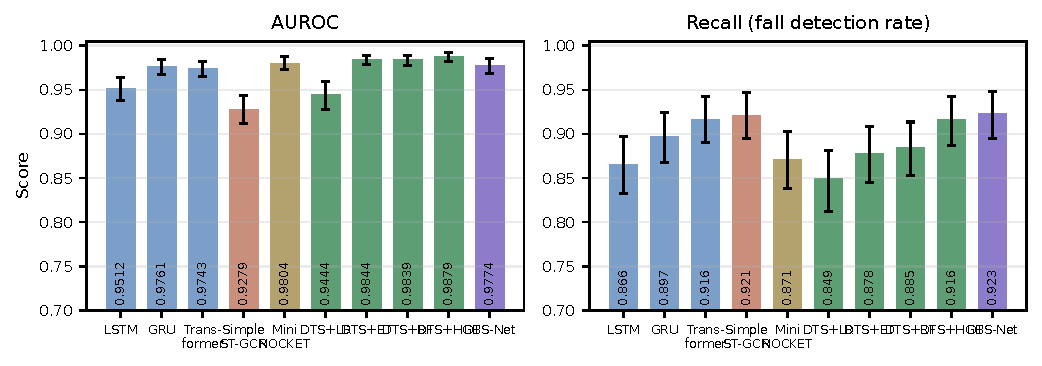
\includegraphics[width=\textwidth]{fig1_main.pdf}
\caption{FallVision held-out AUROC (left) and recall (right) by model with 95\% confidence intervals on the strict twin-free test split. Both panels share the same y-axis range. DTS+HGB is the top AUROC model; the recall panel shows each model at its validation-F1-optimal threshold.}
\label{fig:main}
\end{figure*}

\subsection{Sample Efficiency on Real Data}
The data-scarcity claim is tested directly by retraining the three strongest model families on stratified subsamples of the strict twin-free training set ($n \in \{250, 500, 1{,}000, 2{,}000, 3{,}565\}$; validation, test set, and protocol unchanged). Figure~\ref{fig:lc} shows that DTS+HGB attains the highest test AUROC at every training size: at $n=250$ it reaches 0.9471 versus 0.9360 for the Transformer and 0.9296 for MiniROCKET, and its margin over MiniROCKET is largest in the scarcest regimes ($+0.018$ to $+0.021$ for $n \leq 500$) while persisting at full size ($+0.0135$). The ordering predicted by the capacity argument of Proposition~3 therefore holds on real data along the entire curve, not only at the benchmark's native size.

\begin{figure}[t]
\centering
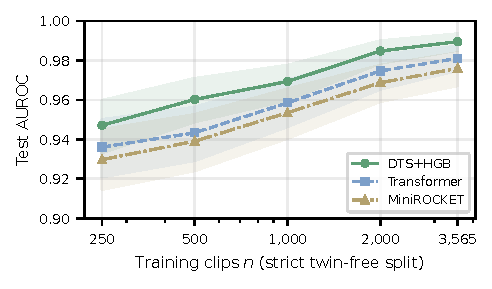
\includegraphics[width=\columnwidth]{fig5_lc.pdf}
\caption{Sample efficiency on the strict twin-free split: test AUROC versus training-set size for the strongest three model families (shaded bands are 95\% bootstrap intervals; validation and test sets fixed). DTS+HGB leads at every size, with the largest margins at the smallest $n$.}
\label{fig:lc}
\end{figure}

\subsection{Leave-Session-Out Evaluation}
Because FallVision does not publish subject IDs, we use the four archive-derived session identifiers as a conservative subject proxy in a leave-one-session-out protocol over the 5{,}572 deduplicated clips (fixed threshold 0.5). DTS+HGB achieves mean AUROC \lsomeanauroc{} (range \lsorangelow--\lsorangehigh) and mean F1 \lsomeanf{} (Table~\ref{tab:lso}, Figure~\ref{fig:lso}), indicating that the main result is not a within-session artefact.

\begin{table}[t]
\centering
\scriptsize
\setlength{\tabcolsep}{2.5pt}
\begin{tabular}{lrrccc}
\toprule
Session & $n$ & Falls & F1 & AUROC & Recall \\
\midrule
1 & \lsoOnen & \lsoOnefalls & \lsoOnef{} \lsoOnefCI & \lsoOneauroc{} \lsoOneaurocCI & \lsoOnerec \\
2 & \lsoTwon & \lsoTwofalls & \lsoTwof{} \lsoTwofCI & \lsoTwoauroc{} \lsoTwoaurocCI & \lsoTworec \\
3 & \lsoThreen & \lsoThreefalls & \lsoThreef{} \lsoThreefCI & \lsoThreeauroc{} \lsoThreeaurocCI & \lsoThreerec \\
4 & \lsoFourn & \lsoFourfalls & \lsoFourf{} \lsoFourfCI & \lsoFourauroc{} \lsoFouraurocCI & \lsoFourrec \\
\midrule
Mean & -- & -- & \lsomeanf & \lsomeanauroc & -- \\
\bottomrule
\end{tabular}
\caption{Leave-session-out evaluation for DTS+HGB (subject proxy; fixed threshold 0.5). Brackets are 95\% bootstrap confidence intervals.}
\label{tab:lso}
\end{table}

\begin{figure}[t]
\centering
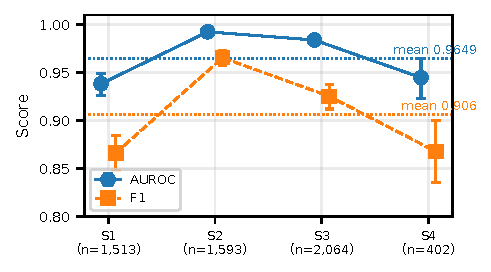
\includegraphics[width=\columnwidth]{fig2_lso.pdf}
\caption{Leave-session-out AUROC and F1 across archive-derived session folds with 95\% confidence intervals. Dotted lines mark the means.}
\label{fig:lso}
\end{figure}

\subsection{Leave-Fall-Origin Robustness}
Table~\ref{tab:lfo} and Figure~\ref{fig:lfo} report acquisition-group robustness on the 5{,}572 deduplicated clips with a fixed threshold of 0.5. The Bed fold (AUROC \lfoBedauroc) is substantially harder: Bed falls begin from a semi-reclined posture with a shorter vertical descent, shifting $\hat{\mu}_f$ and $\hat{\sigma}_f$ outside the Chair+Stand training support, so increased error on this fold is a structural prediction of the QDA model rather than an unexplained failure. Chair and Stand transfer readily. The transfer gap is $\Gamma_{F1} = \iidreff - \lfomeanf = \transfergap$, computed against a stratified iid reference under the same protocol.

\begin{table}[t]
\centering
\scriptsize
\setlength{\tabcolsep}{2.5pt}
\begin{tabular}{lrrcc}
\toprule
Held-out & $n$ & Falls & F1 & AUROC \\
\midrule
Bed & \lfoBedn & \lfoBedfalls & \lfoBedf{} \lfoBedfCI & \lfoBedauroc{} \lfoBedaurocCI \\
Chair & \lfoChairn & \lfoChairfalls & \lfoChairf{} \lfoChairfCI & \lfoChairauroc{} \lfoChairaurocCI \\
Stand & \lfoStandn & \lfoStandfalls & \lfoStandf{} \lfoStandfCI & \lfoStandauroc{} \lfoStandaurocCI \\
\midrule
Mean & -- & -- & \lfomeanf & \lfomeanauroc \\
\bottomrule
\end{tabular}
\caption{Leave-fall-origin robustness for DTS+HGB (fixed threshold 0.5). Brackets are 95\% bootstrap confidence intervals.}
\label{tab:lfo}
\end{table}

\begin{figure*}[t]
\centering
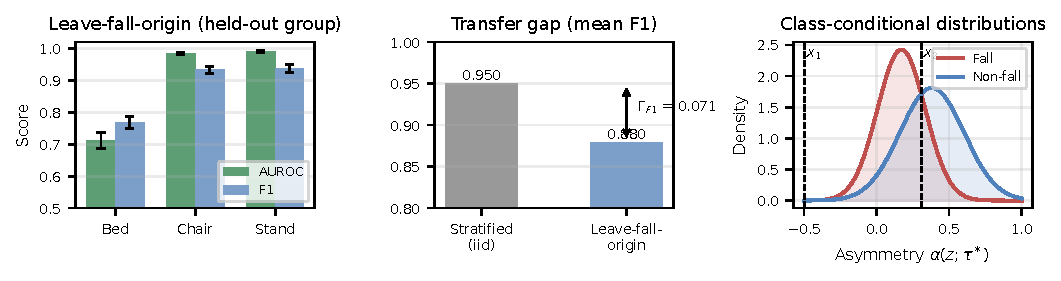
\includegraphics[width=\textwidth]{fig3_lfo.pdf}
\caption{Left: leave-fall-origin AUROC and F1 by held-out acquisition group with 95\% confidence intervals. Centre: transfer gap between the stratified iid reference and the leave-fall-origin mean under the same protocol. Right: class-conditional distributions of hip-speed asymmetry with QDA decision boundaries at $x_1 \approx \xone$ and $x_2 \approx \xtwo$; since $\alpha \geq 0$, only $x_2$ is active.}
\label{fig:lfo}
\end{figure*}

\subsection{Zero-Shot URFD Transfer}
DTS+HGB trained on FallVision and applied to URFD without retraining obtains AUROC \urfdauroc{} \urfdaurocCI{} and recall \urfdrec{} \urfdrecCI, detecting all 30 URFD falls at the fixed threshold (Table~\ref{tab:urfd}). This transfer experiment uses the archived FallVision-trained model; it is unaffected by FallVision-internal duplication because URFD is an external test set. The \urfdfp{} false positives reflect a score-calibration shift rather than poor ranking, since AUROC remains high; precision is \urfdprec{} \urfdprecCI. Recalibrating the threshold on a small number of URFD non-fall samples is expected to reduce false positives substantially.

\begin{table}[t]
\centering
\scriptsize
\setlength{\tabcolsep}{4pt}
\begin{tabular}{lcc}
\toprule
Metric & FallVision (test) & URFD (zero-shot) \\
\midrule
AUROC & \DTSHGBauroc{} \DTSHGBaurocCI & \urfdauroc{} \urfdaurocCI \\
Recall & \DTSHGBrec{} \DTSHGBrecCI & \urfdrec{} \urfdrecCI \\
Precision & \DTSHGBprec{} \DTSHGBprecCI & \urfdprec{} \urfdprecCI \\
F1 & \DTSHGBf{} \DTSHGBfCI & \urfdf{} \urfdfCI \\
FN & \DTSHGBfn & \urfdfn \\
FP & \DTSHGBfp & \urfdfp \\
\bottomrule
\end{tabular}
\caption{Zero-shot cross-dataset transfer (FallVision$\to$URFD, 70 clips, fixed threshold 0.5). Brackets are 95\% confidence intervals; FP and FN are deterministic counts.}
\label{tab:urfd}
\end{table}

\begin{table}[t]
\centering
\scriptsize
\setlength{\tabcolsep}{4pt}
\begin{tabular}{lcccc}
\toprule
Configuration & F1 & AUROC & $\Delta$F1 & $\Delta$AUC \\
\midrule
Full model & \abFullf & \abFullauroc & -- & -- \\
$-$BBox-W & \abBBoxWf & \abBBoxWauroc & \abBBoxWdf & \abBBoxWda \\
$-$Hip-Y & \abHipYf & \abHipYauroc & \abHipYdf & \abHipYda \\
$-$Torso-Ang & \abTorsoAngf & \abTorsoAngauroc & \abTorsoAngdf & \abTorsoAngda \\
$-$Hip-Spd & \abHipSpdf & \abHipSpdauroc & \abHipSpddf & \abHipSpdda \\
$-$Ctr-Spd & \abCtrSpdf & \abCtrSpdauroc & \abCtrSpddf & \abCtrSpdda \\
$-$Hip-Acc & \abHipAccf & \abHipAccauroc & \abHipAccdf & \abHipAccda \\
$-$Shldr-Y & \abShldrYf & \abShldrYauroc & \abShldrYdf & \abShldrYda \\
$-$Head-Y & \abHeadYf & \abHeadYauroc & \abHeadYdf & \abHeadYda \\
Asymmetry zeroed ($\alpha{=}0$) & \abStaticf & \abStaticauroc & \abStaticdf & \abStaticda \\
\bottomrule
\end{tabular}
\caption{DTS+HGB feature ablation on the main held-out protocol (each row retrained; threshold re-tuned on validation). Values to three decimals (F1) and four decimals (AUROC).}
\label{tab:ablation}
\end{table}
\subsection{Feature Ablations}
Table~\ref{tab:ablation} reports single-family removal under the main protocol with the selected DTS+HGB configuration retrained per ablation and the threshold re-tuned on validation. No individual family removal causes large degradation (largest AUROC drop: \abHipYda{} for hip height), revealing that the DTS is intentionally over-complete: each family carries partially redundant signal, providing robustness to missing or noisy keypoints. Zeroing all eight asymmetry elements ($\alpha = 0$) changes AUROC by only \abStaticda{} and F1 by \abStaticdf{} on FallVision, because the remaining temporal operators (slopes, velocities, accelerations) absorb much of the ordering signal on real data; the controlled temporal-order benchmark below isolates the pure ordering contribution that this ablation cannot.



\subsection{Validated Interpretability (DTS-Net)}
DTS-Net attention weights, averaged over five seeds (per-family standard deviation $< 0.03$), correlate positively with ExtraTrees family importances ($r = \attnr$), although with only eight families the correlation does not reach significance ($p = \attnp$). Both methods rank head height (attention \attntopw; importance \attntopei) and shoulder height (\attnsecw; \attnsecei) among the most informative families, consistent with clinical literature identifying upper-body kinematics as early fall indicators.

\subsection{Controlled Temporal-Order Benchmark}
This benchmark is synthetic by design: 600 fall sequences with a three-phase hip trajectory (still, drop, floor), each paired with a non-fall created by randomly permuting its frames, so class marginals are identical multisets by construction and only temporal ordering differs; splits are at the pair level. DTS+HGB attains AUROC \synthdtsathundred{} at $n = 100$ and 1.000 for $n \geq 500$ (5-fold CV \synthcv), while an order-invariant bag-of-frames classifier stays exactly at chance for every $n$, its features being provably identical across classes. Logistic regression on the eight asymmetry values alone reaches AUROC $\geq \synthalphamin$ (Figure~\ref{fig:synth}, left).

\begin{figure*}[t]
\centering
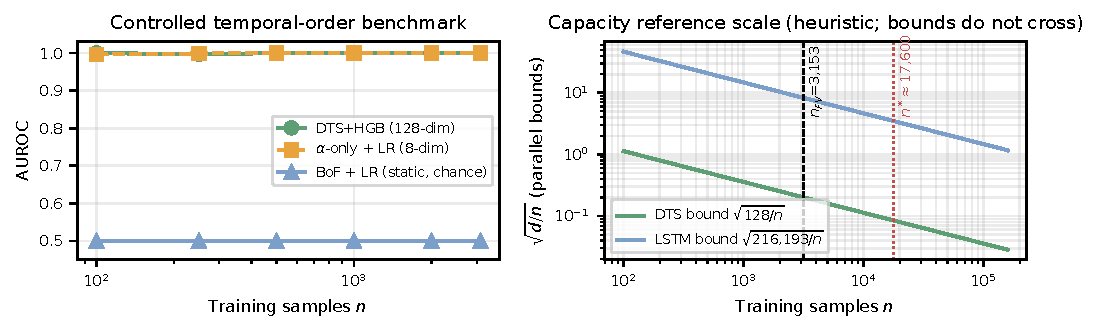
\includegraphics[width=\textwidth]{fig4_synth.pdf}
\caption{Left: controlled temporal-order benchmark; DTS+HGB saturates while order-invariant bag-of-frames features remain exactly at chance (identical marginals by construction). Right: heuristic capacity comparison; the $\sqrt{d/n}$ bounds are parallel and do not cross, $n^* \approx \nstar$ (dotted) is a derived reference scale, and $n_{\mathrm{train}} = \trainn$ (dashed) lies well below it.}
\label{fig:synth}
\end{figure*}

\section{Discussion}
\textbf{When can principled feature engineering beat neural learning?} Proposition~3 suggests three conditions: the task structure is formally characterisable; training data are scarce relative to model capacity; and the feature inductive bias is aligned with the true mechanism. All three hold here, and the evidence is consistent without overstatement: the best DTS ensemble achieves higher AUROC than every evaluated neural, graph, and convolutional baseline at every training size, with paired-bootstrap differences that exclude zero. We do not claim this extends to large-scale multi-class benchmarks or pretrained systems, where the conditions for deep dominance may be restored.

\textbf{Threshold trade-offs.} At validation-F1 thresholds, DTS+HGB misses \DTSHGBfn{} falls and MiniROCKET misses \MiniROCKETfn{} with similar false-positive counts, and the matched-threshold analysis favours DTS at both constraints; deployment should still choose the operating point from the recall-precision curve.

\textbf{Bed fold: predicted, quantified, and partially recoverable.} The hardest robustness fold (Bed, AUROC \lfoBedauroc) is predicted by the QDA model: semi-reclined falls shift the class-conditional asymmetry parameters outside the training support. A few-shot adaptation experiment quantifies the remedy: adding $K$ labelled Bed clips to the Chair+Stand training set (fixed 1{,}547-clip Bed evaluation set) raises AUROC from 0.714 at $K{=}0$ to 0.784 at $K{=}50$ and 0.848 at $K{=}200$, so modest target-domain collection recovers much of the gap. The \urfdfp{} URFD false positives at threshold 0.5 likewise reflect a calibration shift rather than ranking failure (AUROC \urfdauroc); deployment on a new domain requires threshold calibration, which we quantify rather than treat as solved.

\textbf{Deployment efficiency.} DTS extraction and HGB inference total under 3\,ms per clip on commodity CPU with under 50\,MB of memory, compatible with any upstream pose estimator.

\section{Limitations}
\textbf{Erratum.} An earlier draft reported near-ceiling results (AUROC 0.9998, recall 1.000) traced to duplicated clips leaking across splits; all numbers here use the strict twin-free protocol, with full artefacts (code, features, manifests, dedup audit, score vectors, grids, thresholds) released. \textbf{Subject identity.} Leave-session-out is a proxy; sessions may not map one-to-one to subjects. \textbf{Graph/video baselines.} Compact and full COCO-adapted ST-GCNs are trained from scratch; PoseC3D and pretrained systems are not evaluated, so this is an evaluated-baseline comparison, not a state-of-the-art claim. \textbf{Domain shift.} Bed-origin falls remain hardest (AUROC \lfoBedauroc) and URFD transfer needs threshold calibration; both are quantified, not solved. \textbf{Population.} Subjects are healthy adults aged 22--27. \textbf{Scope.} The sub-3\,ms runtime excludes pose estimation; the attention-importance correlation is positive but not significant ($k{=}8$ families).

\section{Conclusion}
Formally characterising fall kinematics through the temporal asymmetry operator $\alpha(z;\tau^*)$ yields a 128-dimensional representation whose single-primitive Bayes bound ($\varepsilon^*_{\mathrm{QDA}} = \epsqda$) the full DTS reduces by a factor of 5.6. Under a strict twin-free protocol with validation-only tuning and confidence intervals on every result, DTS+HGB attains the highest AUROC among eleven evaluated models (\DTSHGBauroc{} \DTSHGBaurocCI), leads at every training-set size, and transfers zero-shot to URFD with recall \urfdrec; a controlled temporal-order benchmark isolates temporal ordering as the signal. When the task mechanism is known and data are scarce relative to model capacity, a theoretically aligned temporal statistic offers a better bias-variance trade-off than generic sequence learning.

\bibliography{references}

\end{document}
